\subsubsection{UC16 - Cronologia di esecuzione}
\begin{figure}[H]
	\centering
	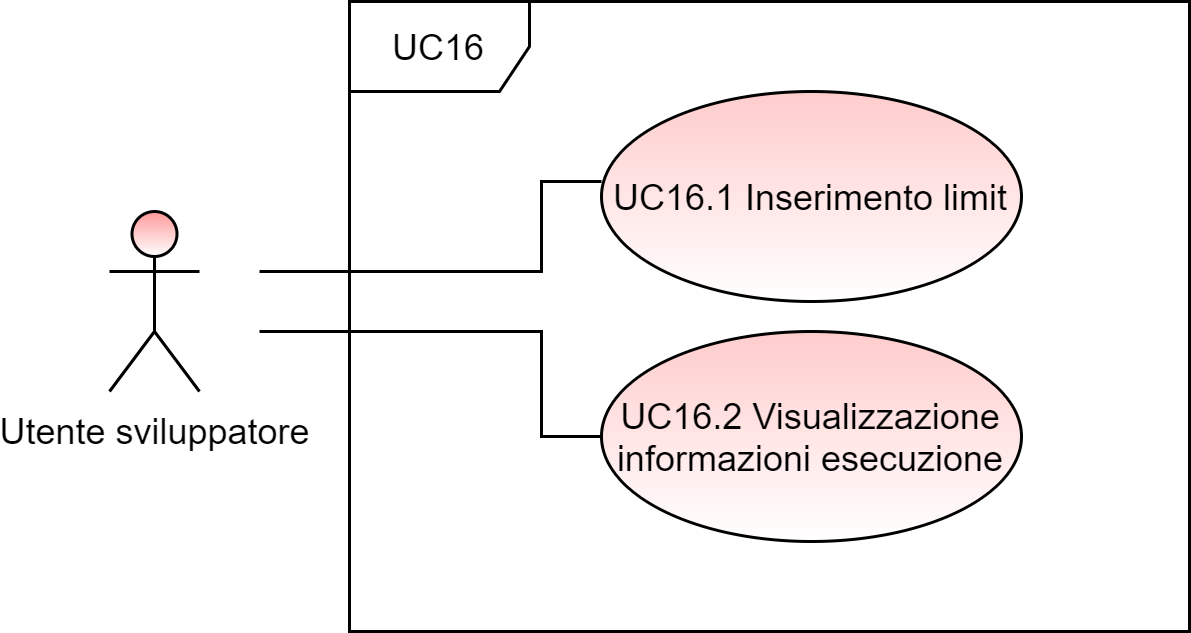
\includegraphics[scale=\ucs]{./res/img/UC16.png}
	\caption {UC16 - Cronologia di esecuzione}
\end{figure}
\begin{itemize}
	\item \textbf{Attori primari:} \us{};
	\item \textbf{Attori secondari:} \re{};
	\item \textbf{Descrizione:} l’utente ottiene le informazioni relative alla propria cronologia di invocazione di funzioni;
	\item \textbf{Scenario principale:} 
	\begin{itemize}
		\item l'utente inserisce il comando \history;  
		\item vengono visualizzate le informazioni relative alla cronologia delle chiamate dell’utente.
	\end{itemize}
	\item \textbf{Estensioni:} 
	\begin{itemize}
		\item \textbf{UC17:} nel caso l’utente non abbia mai eseguito alcuna funzione all’interno della piattaforma viene mostrato un apposito avviso.  
	\end{itemize}
	\item \textbf{Precondizione:} l’utente desidera visualizzare la propria cronologia di utilizzo della piattaforma \textit{Etherless}; 
	\item \textbf{Postcondizione:} viene visualizzata la cronologia di chiamate dell’utente.  
\end{itemize}